% ==========================================
% Section 11: Sampling Strategies (Slides 52-57)
% ==========================================

% Slide 52: Sampling Revisited
\begin{frame}{نمونه‌گیری مجدد (\lr{Sampling Revisited})}
\begin{itemize}
  \item \textbf{کاهش عرض در برابر کاهش ارتفاع مجموعه داده:}
  \begin{itemize}
    \item انتخاب زیرمجموعه ویژگی‌ها عرض داده‌ها (تعداد ستون‌ها) را کاهش می‌دهد.
    \item نمونه‌گیری ارتفاع داده‌ها (تعداد سطرها / رکوردها) را کاهش می‌دهد.
  \end{itemize}
  \vspace{0.3cm}
  \item \textbf{چرا نمونه‌گیری انجام می‌دهیم؟}
  \begin{itemize}
    \item حجم داده‌ها بسیار فراتر از حافظه در دسترس است.
    \item آزمایش و مقایسه سریع‌تر الگوریتم‌های مختلف در مراحل اولیه پروژه.
  \end{itemize}
  \vspace{0.3cm}
  \item \textbf{انواع نمونه‌گیری متداول:}
  \begin{itemize}
    \item نمونه‌گیری تصادفی ساده (\lr{Simple Random Sampling})
    \item نمونه‌گیری طبقه‌بندی‌شده (\lr{Stratified Sampling}) برای حفظ نسبت کلاس‌ها
  \end{itemize}
\end{itemize}
\end{frame}

% Slide 53: Kennard-Stone Sampling
\begin{frame}{الگوریتم نمونه‌گیری کنارد-استون (\lr{Kennard-Stone})}
\begin{columns}[c]
  \begin{column}{0.55\textwidth}
    \begin{itemize}
      \item \textbf{هدف: انتخاب نمونه‌هایی با حداکثر پوشش فضای ویژگی.}
      \vspace{0.2cm}
      \item \textbf{مراحل الگوریتم:}
      \begin{enumerate}
        \item محاسبه فواصل دوبه‌دوی تمام نقاط در فضای ویژگی.
        \item انتخاب دو نقطه‌ای که بیشترین فاصله اقلیدسی را از یکدیگر دارند به عنوان نمونه‌های نخست.
        \item در هر مرحله بعدی، افزودن نقطه‌ای که بیشترین کمینه فاصله را از نقاط انتخاب‌شده قبلی دارد.
      \end{enumerate}
    \end{itemize}
  \end{column}
  \begin{column}{0.43\textwidth}
    \centering
    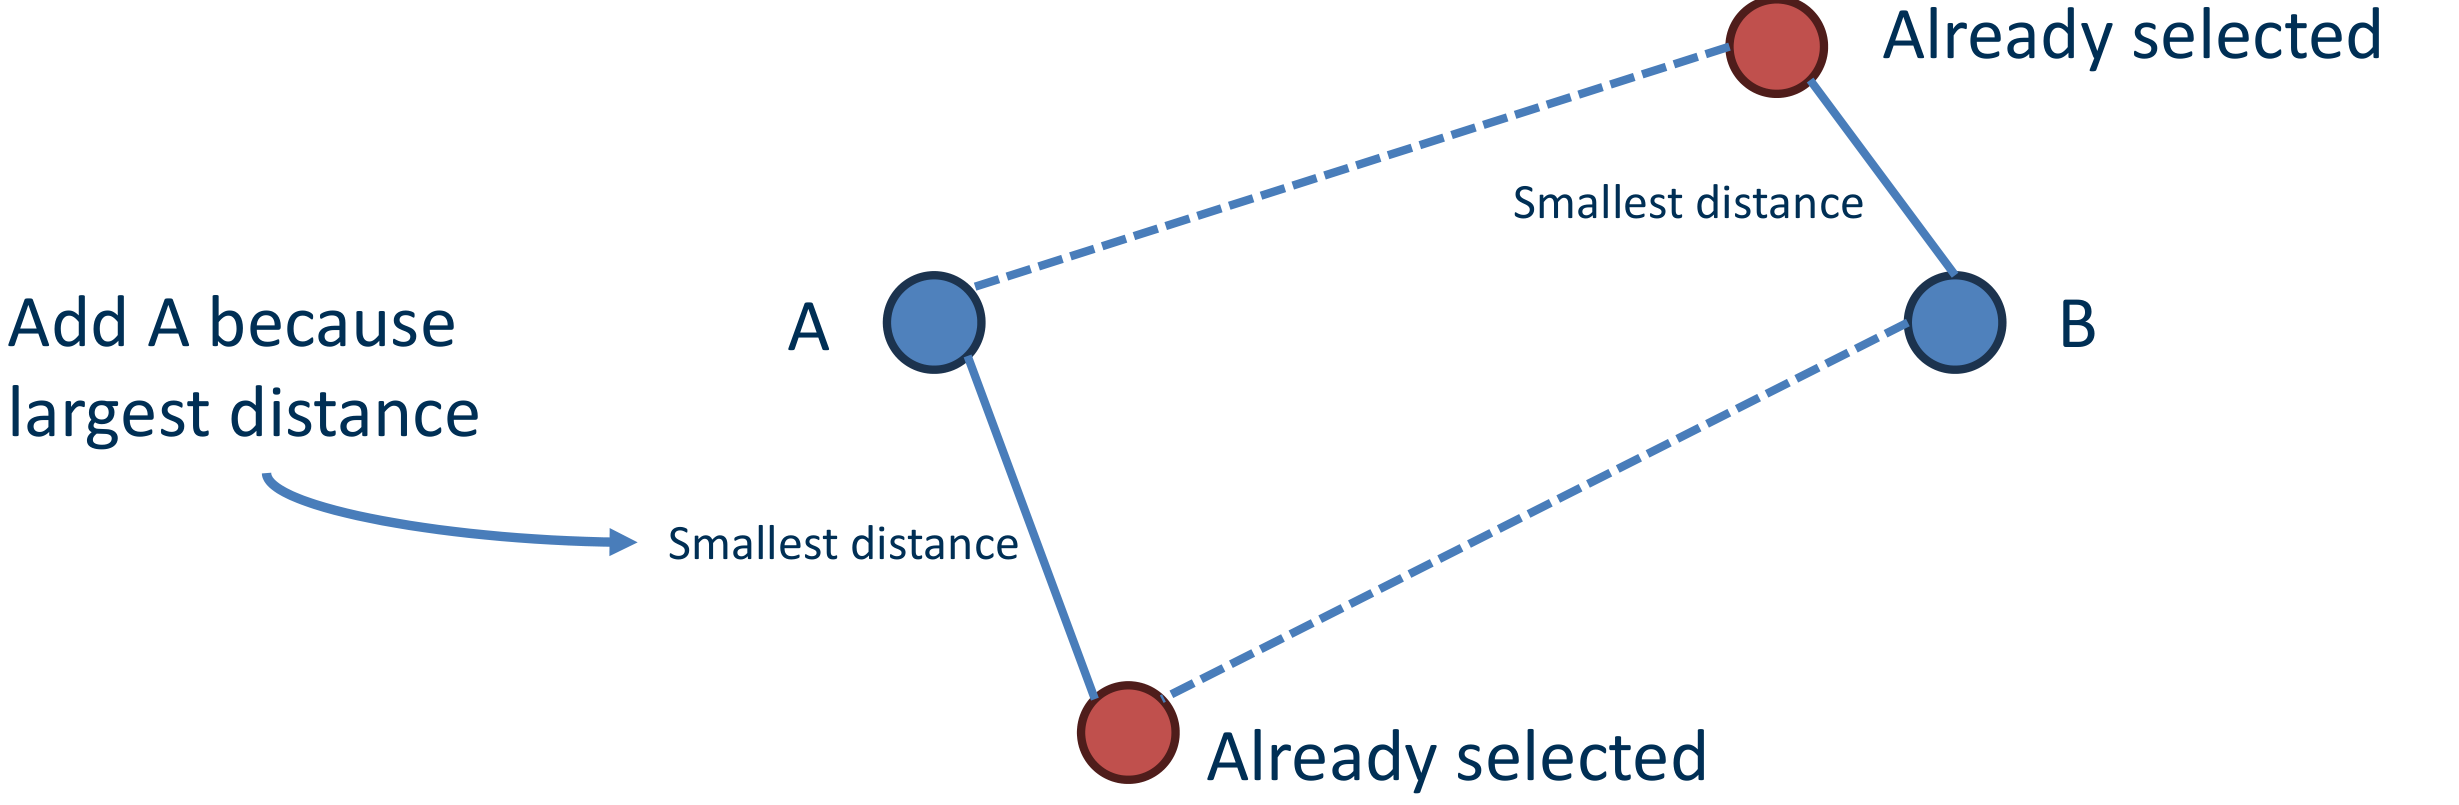
\includegraphics[width=\textwidth]{images/page_53_matrix.png}
  \end{column}
\end{columns}
\end{frame}

% Slide 54: Kennard-Stone Continued
\begin{frame}{الگوریتم کنارد-استون: ویژگی‌ها و پیاده‌سازی}
\begin{itemize}
  \item \textbf{تضمین تنوع نقاط انتخاب‌شده:}
  \begin{itemize}
    \item تضمین می‌کند که نقاط ناهمگن و متنوع به مجموعه نمونه اضافه شوند (افزایش تنوع نمونه‌ها).
    \item پوشش کامل‌تر موارد گوشه‌ای و نادر (\lr{Corner Cases}) در فضای ویژگی‌ها.
    \item اما پتانسیل جذب نقاط غیرعادی و پرت (\lr{Outliers}) نیز به مراتب بیشتر می‌شود.
    \item توزیع احتمالاتی طبیعی داده‌ها ممکن است دستخوش تغییر گردد.
  \end{itemize}
  \vspace{0.3cm}
  \item \textbf{پیاده‌سازی در پایتون (\lr{Python})}
  \begin{itemize}
    \item به طور پیش‌فرض در \lr{scikit-learn} تعبیه نشده است.
    \item نیاز به نصب بسته مستقل \codeinline{kennard-stone}:\\
    \vspace{0.1cm}
    \codebox{pip install kennard-stone}
  \end{itemize}
\end{itemize}
\vspace{0.3cm}
\flushright
{\fontsize{7}{8.5}\selectfont\color{subgray}پیوند مخزن پایتون: \lr{https://pypi.org/project/kennard-stone/}}
\end{frame}

% Slide 55: Kennard-Stone Example
\begin{frame}{مثال عملی نمونه‌گیری کنارد-استون}
\begin{columns}[c]
  \begin{column}{0.55\textwidth}
    \begin{itemize}
      \item \textbf{مزیت (\lr{Pro})}
      \begin{itemize}
        \item بخش زیادی از موارد خاص، غیرعادی و لبه‌ای در نمونه پوشش داده می‌شوند.
      \end{itemize}
      \vspace{0.3cm}
      \item \textbf{عیب (\lr{Con})}
      \begin{itemize}
        \item توزیع احتمالاتی طبیعی داده‌ها به کلی دستخوش تغییر می‌شود.
        \item تمرکز نامتناسبی بر نقاط پرت و مرزی ایجاد می‌گردد.
      \end{itemize}
    \end{itemize}
  \end{column}
  \begin{column}{0.43\textwidth}
    \centering
    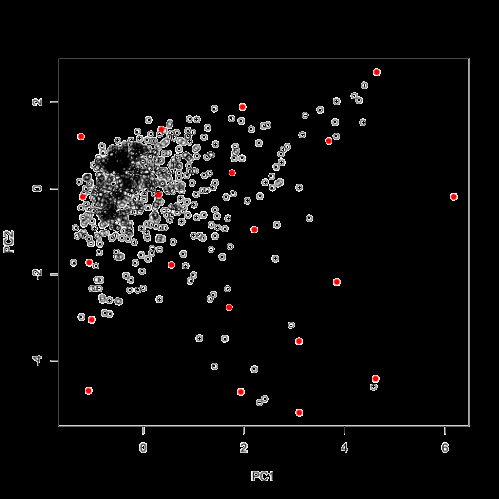
\includegraphics[width=\textwidth]{images/page_55_img_1.png}
  \end{column}
\end{columns}
\end{frame}

% Slide 56: Interaction Effects
\begin{frame}{برهم‌کنش استراتژی‌های نمونه‌گیری با الگوریتم‌ها}
\begin{itemize}
  \item \textbf{اثرات متقابل استراتژی نمونه‌گیری و نوع الگوریتم یادگیرنده:}
  \begin{itemize}
    \item \textbf{مدل‌های متکی بر توزیع آماری (مانند بیز ساده / \lr{Naive Bayes})}
    \begin{itemize}
      \item وابسته به برآورد درست احتمالات؛ نمونه‌گیری طبقه‌بندی‌شده (\lr{Stratified}) کارایی بالاتری دارد.
    \end{itemize}
    \item \textbf{مدل‌های متکی بر مرزهای تفکیک (مانند درخت تصمیم / \lr{Decision Trees})}
    \begin{itemize}
      \item حساسیت کمتر به توزیع کلی؛ پوشش نقاط لبه‌ای با کنارد-استون صحت مدل را بالا می‌برد.
    \end{itemize}
  \end{itemize}
\end{itemize}
\vspace{0.15cm}
\centering
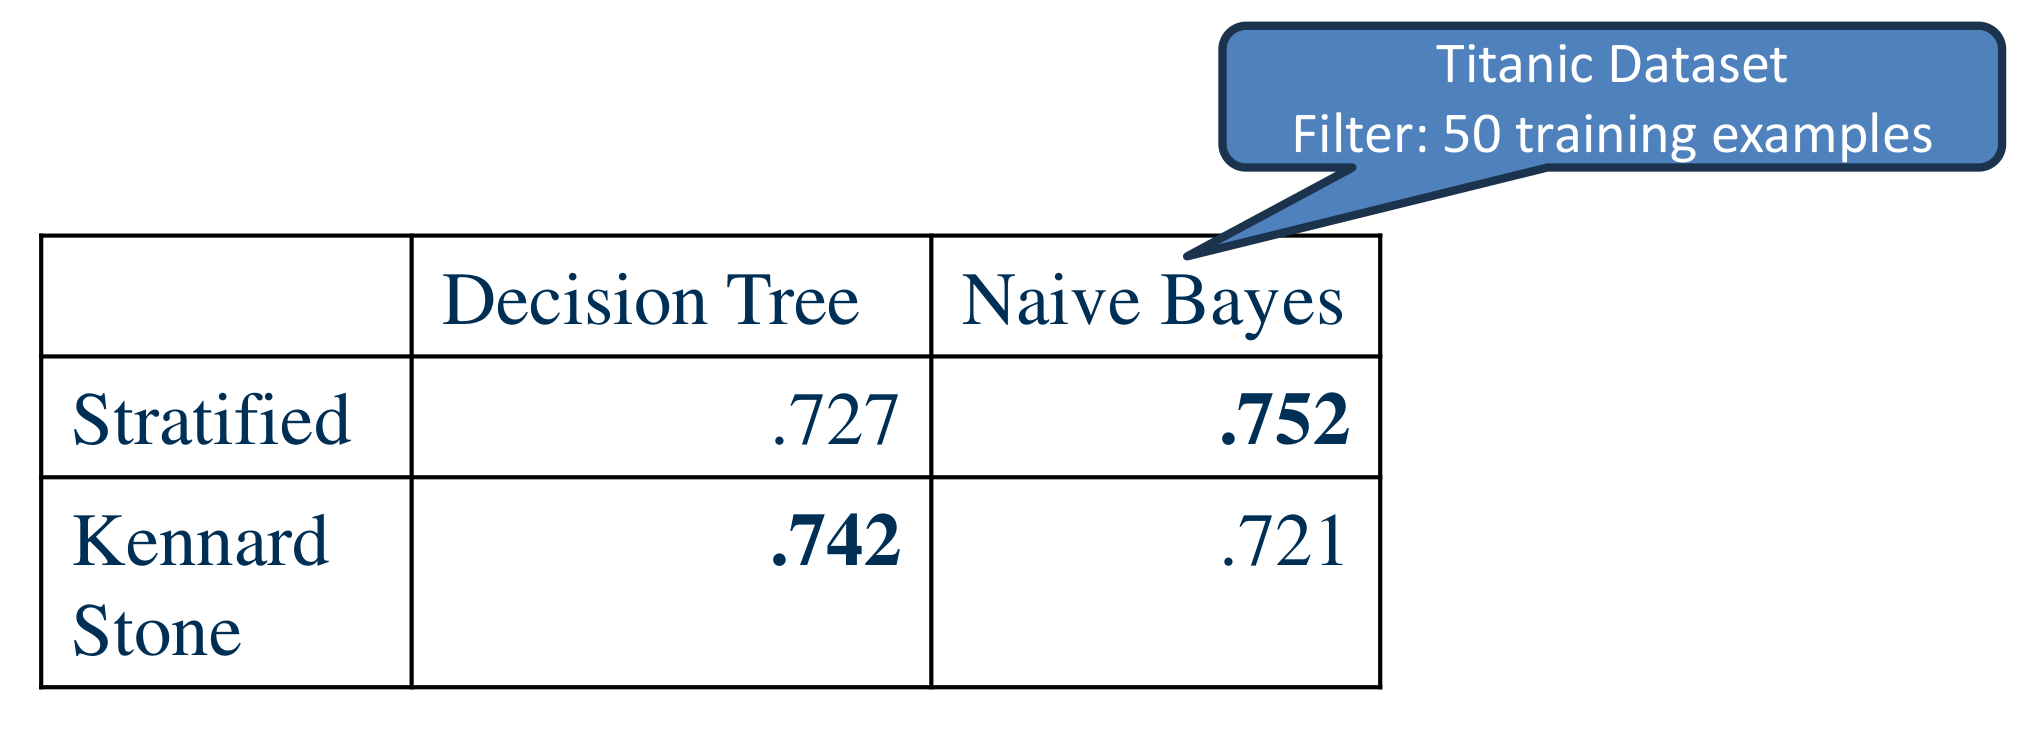
\includegraphics[width=0.62\textwidth]{images/page_56_chart.png}
\end{frame}

% Slide 57: Real-world Note on Sampling
\begin{frame}{نکته‌ای پیرامون نمونه‌گیری در پروژه‌های واقعی}
\begin{itemize}
  \item \textbf{داده‌های آموزشی در پروژه‌های دنیای واقعی غالباً خود یک نمونه هستند:}
  \begin{itemize}
    \item به عنوان نمونه: ارقام فروش ماه گذشته، گزارش‌های مالیاتی سال قبل، یا سوابق بیماران بستری در یک بیمارستان خاص.
  \end{itemize}
  \vspace{0.3cm}
  \item \textbf{پرسش‌های اساسی که همواره باید مد نظر داشت:}
  \begin{itemize}
    \item آیا نمونه فعلی واقعاً نماینده جامعه آماری آینده است؟
    \item آیا پدیده تغییر توزیع داده‌ها در طول زمان (\lr{Data Drift / Concept Drift}) رخ نداده است؟
    \item آیا فرآیند گردآوری داده‌ها ناخواسته دچار سوگیری انتخاب (\lr{Selection Bias}) نبوده است؟
  \end{itemize}
\end{itemize}
\end{frame}
